\section{Split-DASH System Architecture}
The DASH or DASH like system provides a way (guideline) to change video quality instead of pausing a video streaming during bad network quality. There are several implementation of the DASH or DASH like streaming system and most of them have a HTML5 based implementation using {\it Media Source Extension}(MSE)\cite{wiki:dash,w3c:mse}. These implementations also support {\it Digital Right Management}(DRM) via {\it Encrypted Media Extension}(EME)\cite{w3c:eme}. These implementation have several modules implemented either in {\it Javascript} or in browser. The modules like playback, media decryption are implemented in browser or some browser extension/plugin (\ie Widevine plugin for DRM protection). The different modules are as follows:

{\bf Playback module} or the player is the module which actually render the video. It is implemented mostly in the browser. It is mostly implemented in the browser and render in a html element. The player is accessed and controlled via MSE APIs.

{\bf Buffer controller} manages and monitor video buffer. It is partly implemented using javascript and partly by the browser itself.

{\bf Adaptive bitrate controller} is the module decides the quality based on the network condition. It can have multiple algorithm and implemented in javascript it self. It is the most crucial part of DASH like streaming system yet the most flexible part. Any streaming provider can implement there won algorithm based on their requirement. We will discuss more about ABR later part of the article.

{\bf Download manager} is responsible for downloading the segment/chunk chosen by the ABR algorithm. It monitors the progress of ongoing downloads to gain fine tune information about the network condition. Most of the time it download chunk using AJAX (Asynchronous JavaScript And XML)


{\bf CDN/Streaming Servers} are http based static file server. It contains all the data requires to play a video smoothly.

{\bf DRM protection module:} It provides DRM protection using EME when a streaming provider wants to protect the right of content. It is an independent component and does not influence the ABR algorithm or other components. DRM protection module is out of the scope of this work.

\begin{figure}[ht]
   \begin{center}
           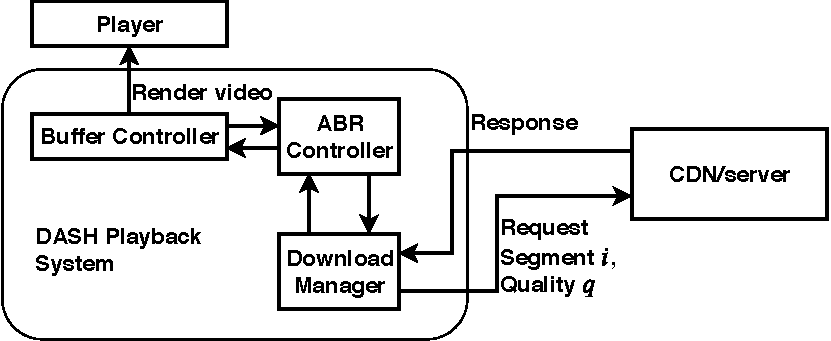
\includegraphics[width=0.7\linewidth]{img/playerDiagram_basic}
   \end{center}
   \caption{\label{fig:playerDiagram_basic} Original DASH based streaming system.}
\end{figure}

The inter-connection of the modules are depicted in the Fig.~\ref{fig:playerDiagram_basic}. Here, the ABR controller controls the playback via buffer controller while instructing download manager to download appropriate segment in the appropriate time. The ABR controller is the most important component. There are active research going on to improve ABR controller. As ABR controller is the part of the player, it need to be implemented in client application it self. In case HTML based player, ABRs need to be implemented in javascript. The ABR algorithm like MPC\cite{dash:mpc}, BOLA\cite{dash:bola} or the algorithms described in \cite{dash:probe,dash:cs2p,dash:CFA,dash:rnb,dash:buffer} does not have any special library requirement and can be implemented easily in any technology. However, as machine learning based ABR algorithm like Pensieve\cite{dash:pensieve}, OBOE\cite{dash:oboe} or HotDASH\cite{dash:hotdash} need specialized machine learning (ML) library and very hard to implement if the technology does not have support for required library. So, it is very difficult to deploy these algorithm in browser based video player.

\begin{figure}[ht]
	\begin{center}
		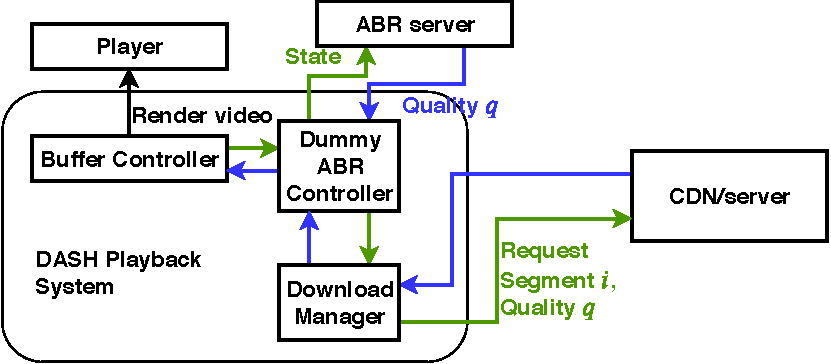
\includegraphics[width=0.7\linewidth]{img/playerDiagram_ml}
	\end{center}
	\caption{\label{fig:playerDiagram_ml} Modified DASH based streaming system to support ML based ABR algorithm}
\end{figure}

Authors of the ML based algorithm show prototype by modifying the system little bit. The new dash based video system looks like Fig.~\ref{fig:playerDiagram_ml}. Here they propose to replace the ABR controller in the client with a dummy one and run a ABR server in the local system. Every time, the player need to take a decision, dummy ABR controller contact ABR server with the current state of the player. The ABR server response the decision based on the algorithm of its choice.

The advantage of this system is that it does not depends on the client technology. ABR server can be implemented in any technology it suit best. However, it involves a extra communication with a external server which may be fatal to the viewing experience if the round trip time between the player and the ABR server. To avoid the communication delay between the player and ABR server, the ABR server need to run in local system only. This system is not easy to deploy as it need to a ABR server of each and every player.

\subsection{Split-DASH architecture}
\label{sec:Split_DASH_architecture}
To solve above problem we propose Split-DASH architecture. In split-DASH architecture, we split the original DASH architecture into two parts, i) a dumb player or client and ii) a smart server side. The proposed architecture depicted in the Fig.~\ref{fig:playerDiagram_split}.
\begin{figure}[ht]
	\begin{center}
		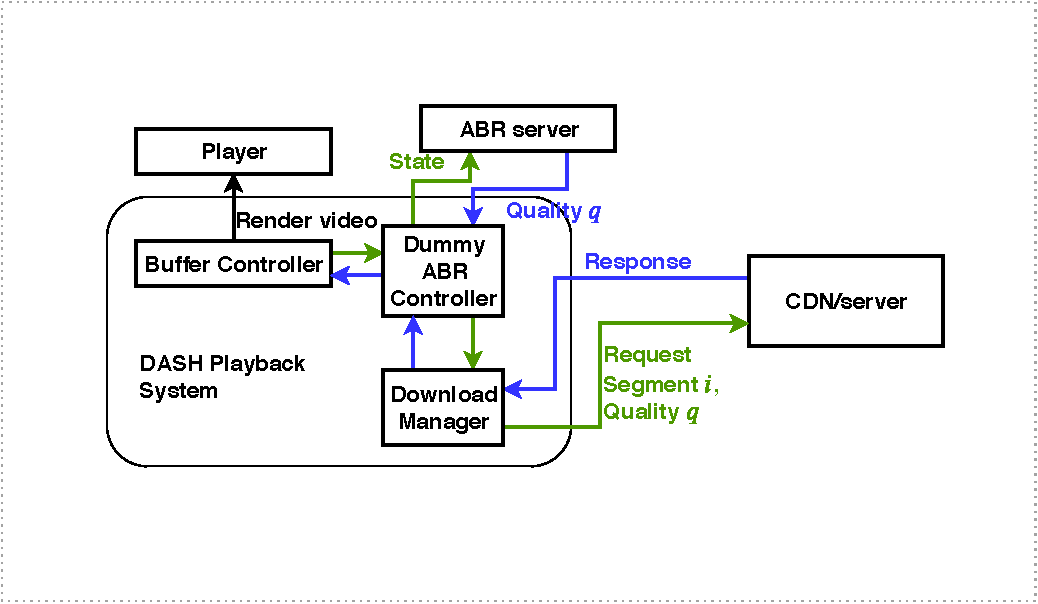
\includegraphics[width=0.9\linewidth]{img/playerDiagram_split}
	\end{center}
	\caption{\label{fig:playerDiagram_split} Modified DASH based streaming system to support ML based ABR algorithm}
\end{figure}
Here we make the player dumb. It controls the play back but it do not take any decision. Instead it depends on the decision provided by the smart part counter part in the server. The server provides the following decision: i) time to download a segment, and ii) quality of the segment. Before we explain functionality of different modules in the server and client, we explain the transaction between dumb-client and the smart server. 

\begin{figure}[h]
	\begin{center}
		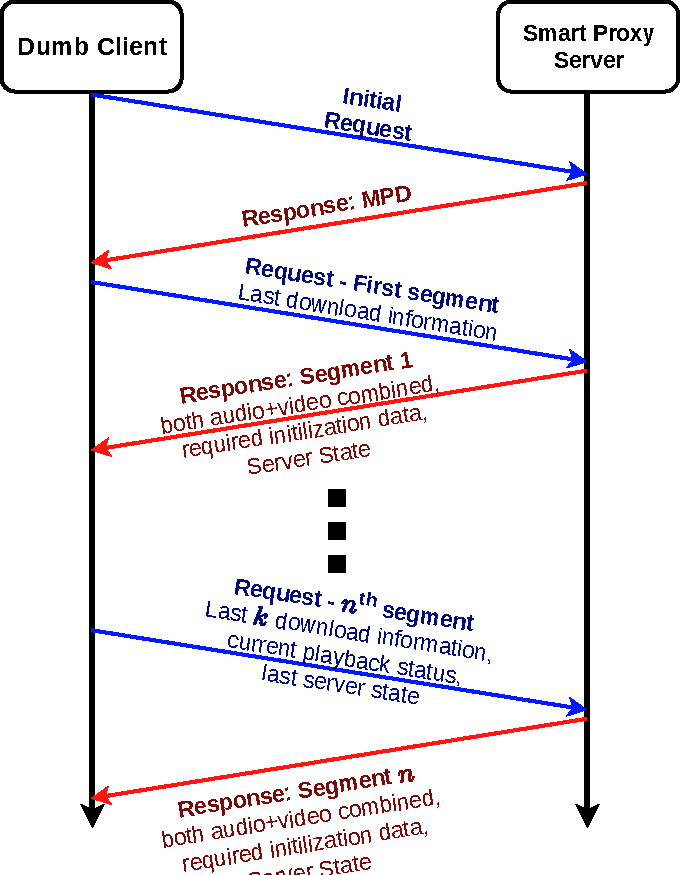
\includegraphics[width=0.5\linewidth]{img/splitDASHTransaction}
	\end{center}
	\caption{\label{fig:splitDASHTransaction} Modified DASH based streaming system to support ML based ABR algorithm}
\end{figure}

The Fig.~\ref{fig:splitDASHTransaction} depict the transaction between smart proxy server and dumb client. At first client request the Media Presentation Description (MPD) from the server. The smart proxy server returns a un-modified MPD for the video. However, it also adds a server identifier {\tt X-Server-Type: Smart}. This identifier indicate that the server is not simple CDN server, instead, it is a smart proxy server. So, the dumb client prepare the HTML video element and request for the first video segment. Here client does not mention the video/audio quality for the segment. Instead, client enclose the download history with the request. When the server receives a request, it looks for old server state in the request. If present, it will expand the state, other wise, it create a new state. Then, update the state according to the current playback information and download history provided in the request. Based on this information, server calculate the best quality for both audio and video segment based on the pre-decided ABR algorithm. Once quality is decided, it download the required segments of the calculated quality from the CDN/streaming (if not available in it cache) and send it back to the dumb player. It Also calculate the time player should wait (i.e. sleep time) before sending another request to the server. It multiplexes the sleep time and server state with the request. The contents of the server state is dependent of the ABR algorithm. Most of the deterministic ABR algorithm, does not required to maintain any state, however, ABR algorithm like pensieve need to maintain state. In case of pensieve, server state contains only the pensieve state.
Here we send server state to client to make server stateless. The client does not read the server state, however, it store it and send with next request.

\noteam{need to add overhead with a table or plot}


\section{SpEnDASH Architecture}
Recently we have developed a energy aware DASH based ABR algorithm EnDASH for smartphones. The algorithm is described in \noteam{cite/ref algo here}. The EnDASH algorithm heavily dependent on smartphone sensor data and neural-network driven ABR algorithm. We implement the EnDASH by modifying Split-DASH architecture (\ref{sec:Split_DASH_architecture}). We call it SpEnDASH architecture. The SpEnDASH architecture have 3 parts, i) A android application, ii) Modified split-DASH dumb client and iii) EnDASH aware smart proxy server. Fig.~\ref{fig:playerDiagram_SpEnDASH} describe the different components and interactions between those components.
%In this model, entire video playback system run inside a webview in an android application. The application collect several informations regarding the device and feed to the webview. The dumb player running inside the webview collect those data and send them to the server with the segment request. The server store those use all the informations to find out the next video quality using the EnDASH algorithm and return the response accordingly.
\begin{figure}[h!]
	\begin{center}
		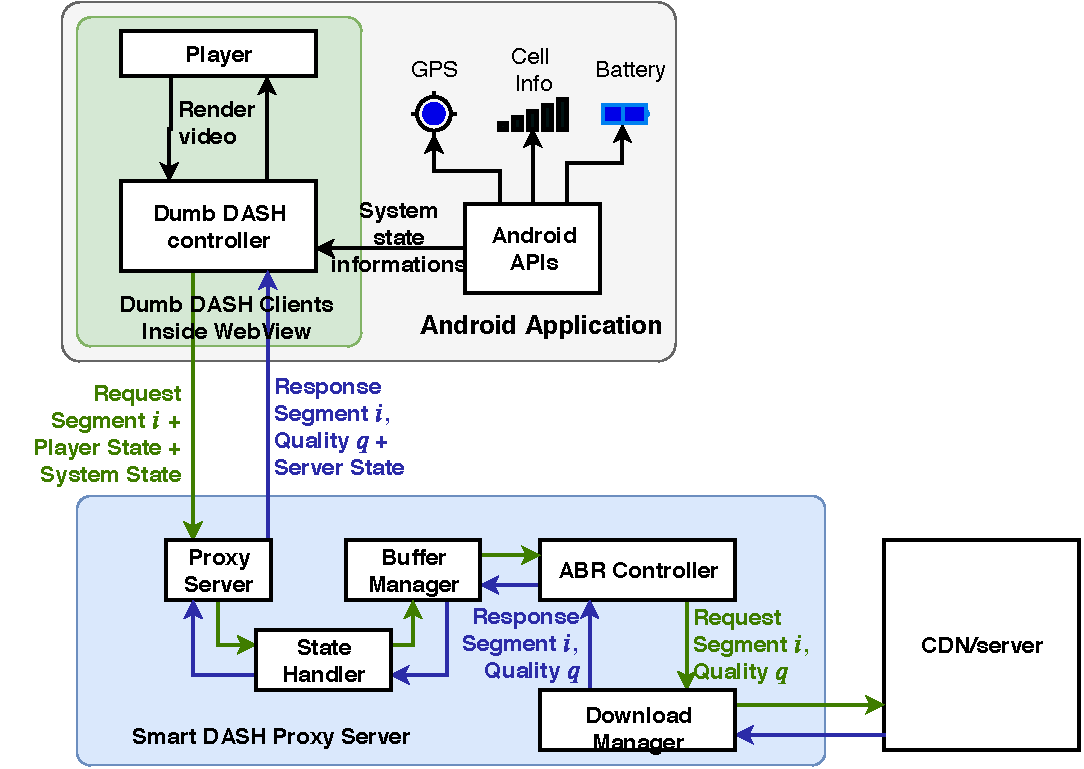
\includegraphics[width=0.9\linewidth]{img/playerDiagram_SpEnDASH}
%		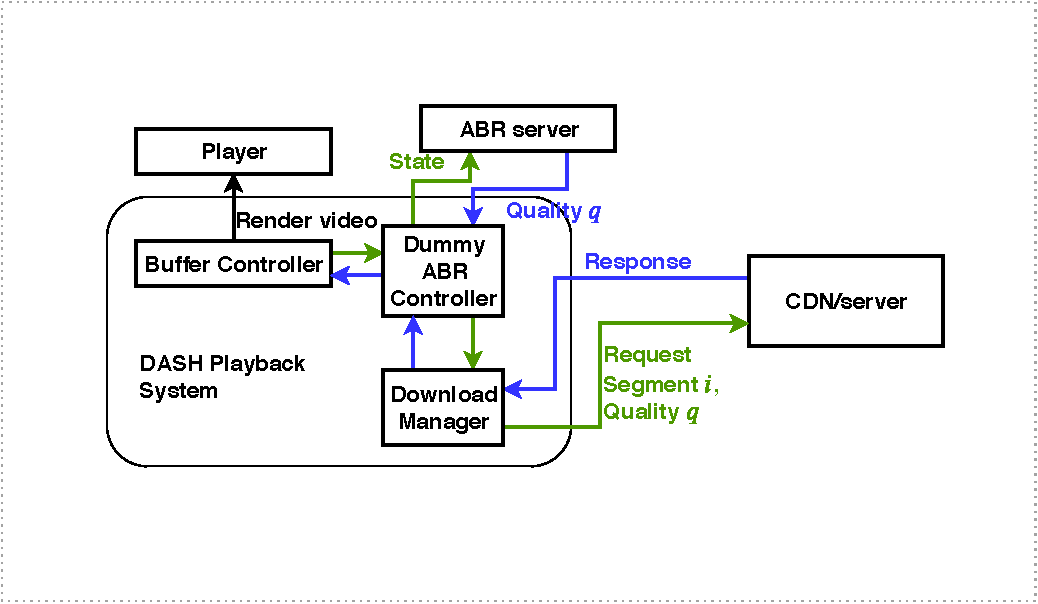
\includegraphics[width=0.9\linewidth]{img/playerDiagram_split}
	\end{center}
	\caption{\label{fig:playerDiagram_SpEnDASH} Modified DASH based streaming system to support ML based ABR algorithm}
\end{figure}
Here we develop a android application.

{\bf Advantages:}